%!TEX root = ../../book_ML.tex
\chapter{Cơ sở lý thuyết}
\label{cha: chap2}
% \index{principal component analysis}
% \index{PCA -- \textit{xem} principle component analysis}
% \index{PCA}

% \index{phân tích thành phần chính -- principle component analysis}
% \index{principle component analysis -- phân tích thành phần chính}
% \index{PCA}
\section{Tổng quan về các kĩ thuật nén mất mát thông tin}
Trong công nghệ thông tin, nén mất mát thông tin hoặc nén không thể đảo
ngược là lớp phương pháp mã hóa dữ liệu sử dụng các phép gần đúng
và loại bỏ một phần dữ liệu để thể hiện nội dung. Các kỹ thuật này
được sử dụng để giảm kích thước dữ liệu để lưu trữ, xử lý và truyền
tải nội dung. Công nghệ nén mất dữ liệu được thiết kế tốt thường
làm giảm kích thước tệp đáng kể trước khi người dùng cuối nhận
thấy sự xuống cấp.

Nén mất dữ liệu được sử dụng phổ biến nhất để nén dữ liệu
đa phương tiện (âm thanh, video và hình ảnh), đặc biệt trong
các ứng dụng như phương tiện truyền trực tiếp hoặc điện thoại internet.

Để mô tả định lượng mức độ gần đúng của dữ liệu tái tạo so
với dữ liệu gốc, cần có một số hình thức đo độ biến dạng.
Vậy nên, trước khi tìm hiểu về các thuật toán nén mất dữ
liệu thường sử dụng, chúng ta cần quan tâm đến một số hình
thức đo độ biến dạng.

Một phép đo sự biến dạng là 1 đại lượng toán học chỉ mức
độ gần đúng so với giá trị ban đầu của nó sử dụng một số
tiêu chí biến dạng. Khi nhìn vào dữ liệu đã nén, người ta
thường nghĩ về sự khác biệt số giữa dữ liệu gốc và dữ liệu
được tái tạo. Tuy nhiên, khi dữ liệu được nén là một ảnh,
phép đo như vậy có thể không mang lại một kết quả như mong muốn.

Ví dụ: nếu hình ảnh được tái tạo giống với ảnh gốc ngoại
trừ việc nó bị lệch sang phải bởi một đường quét dọc, thì
một người quan sát bình thường sẽ gặp khó khăn trong việc
phân biệt nó với ảnh gốc và do đó sẽ kết luận rằng sự biến
dạng nhỏ. Tuy nhiên, khi tính toán được thực hiện bằng số,
chúng ta nhận thấy sự biến dạng lớn, do những thay đổi lớn
trong các pixel riêng lẻ của ảnh được tái tạo. Vấn đề là
chúng ta cần một phép đo về sự biến đổi cảm giác, chứ không
phải một phương pháp số học ngờ nghệch.

Trong số rất nhiều phép đo biến dạng cảm giác đã được tìm ra,
chúng ta trình bày ba phép đo phổ biến nhất được sử dụng
trong nén hình ảnh. Nếu chúng ta quan tâm đến sự khác nhau
pixel trung bình, thì sai số bình phương(MSE- Mean square error)
$\sigma^2$ thường được sử dụng:

\begin{equation}
    \sigma^2 =  \frac{1}{N} \sum_{n=1}^{N} {\left( {X_n-Y_n} \right)}^2
\end{equation}

Với $X_n$, $Y_n$, $N$ lần lượt là chuỗi dữ liệu vào, chuỗi dữ liệu phục hồi,
độ dài của chuỗi dữ liệu

\section{Các kĩ thuật nén codec thường được sử dụng}


Mã hóa biến đổi(Transform coding), một số hình thức nén mất dữ liệu có thể được coi là ứng dụng
của mã hóa biến đổi , là một kiểu nén dữ liệu được sử dụng cho
hình ảnh kỹ thuật số tín hiệu , âm thanh kỹ thuật số và video kỹ thuật số .

Việc chuyển đổi thường được sử dụng để cho phép lượng tử
hóa tốt hơn (nhắm mục tiêu hơn). Kiến thức về ứng dụng được
sử dụng để chọn thông tin cần loại bỏ, do đó làm giảm băng
thông của nó. Thông tin còn lại sau đó có thể được nén thông
qua nhiều phương pháp. Khi đầu ra được giải mã, kết quả có
thể không giống với đầu vào ban đầu, nhưng được mong đợi là
đủ gần với mục đích của ứng dụng.

\subsection{Phương pháp biến đổi Cosin rời rạc}

Biến đổi Cosin rời rạc (Discrete Cosine Transform - DCT)
là một kỹ thuật mã hóa biến đổi được sử dụng rộng rãi,
có khả năng thực hiện mối tương quan của tín hiệu đầu vào
theo cách độc lập với dữ liệu.

Nguyên tắc chính của phương pháp mã hóa này là biến đổi các
giá trị pixel của ảnh trong miền không gian sang một tập các
giá trị khác trong miền tần số, sao cho các hệ số trong tập giá
trị mới này có tương quan giữa các điểm ảnh gần nhau nhỏ hơn.

\begin{figure}
    \begin{subfigure}{0.8\textwidth}
        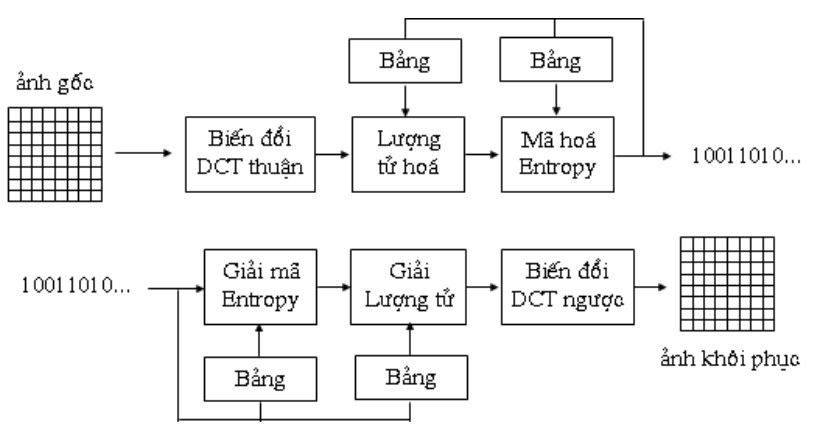
\includegraphics[width=1.0\linewidth]{Chapters/items/DCT.jpg}
         
        \label{fig: dct}
    \end{subfigure}
    \caption{Sơ đồ mã hóa, giải mã sử dụng DCT}
\end{figure}

\subsubsection{Giải thích DCT}
Cho một hàm f(i,j) với 2 biến số nguyên i và j (là thành phần của ảnh),
DCT 2 chiều biến đổi nó sang một hàm mới F(u,v) với u, v chạy trên
cùng một phạm vi với i và j.

Công thức chung cho phép biến đổi là:
\begin{equation*}
    \mathbf{F}_{(u,v)} = \frac{C(u)}{\sqrt{N/2}} \frac{C(v)}{\sqrt{N/2}} \sum_{i=0}^{N-1} \sum_{j=0}^{N-1}  \cos \frac{(2i+1)u\pi}{2N} \cos\frac{(2j+1)v\pi}{2N} \mathbf{f}_{(i,j)}
\end{equation*}

Trong đó ${C(u)}$ và ${C(v)}$ được xác định bởi:

\begin{equation*}
    C(u) = \begin{cases} \frac{1}{\sqrt{2}} & u = 0 \\ 1 & u>0 \end{cases}\text{.}
\end{equation*}

Biến đổi DCT nghịch:
\begin{equation*}
    \mathbf{\tilde{f}}_{(i,j)} = \frac{C(u)}{\sqrt{N/2}} \frac{C(v)}{\sqrt{N/2}} \sum_{i=0}^{N-1} \sum_{j=0}^{N-1}  \cos \frac{(2i+1)u\pi}{2N} \cos\frac{(2j+1)v\pi}{2N} \mathbf{F}_{(u,v)}
\end{equation*}

Trong tiêu chuẩn nén ảnh JPEG, một khối ảnh được xác định có kích thước N = 8.
Các phép biến đổi 2D có thể áp dụng cho các tín hiệu 2D, chẳng hạn như ảnh kỹ
thuật số.



\subsection{Biến đổi Karhunen-Loeve}

Phép biến đổi Karhunen-Loeve (KLT) là một phép biến đổi tuyến tính
có thể đảo ngược khai thác các đặc tính thống kê của biểu diễn vectơ.
Thuộc tính chính của nó là nó trang trí tối ưu đầu vào. Để làm như vậy,
nó phù hợp với một ellipsoid n chiều xung quanh dữ liệu (trung bình đã trừ).
Trục ellipsoid chính là hướng thay đổi chính của dữ liệu.

Hãy nghĩ về một điếu xì gà không may bị giẫm phải. Dữ liệu xì
gà bao gồm một đám mây điểm trong không gian 3 cung cấp tọa độ vị trí của các điểm đo được trong điếu xì gà. Trục dài của điếu xì gà sẽ được xác định bởi một chương trình thống kê là trục KLT đầu tiên.

Trục quan trọng thứ hai là trục nằm ngang qua điếu xì gà bẹp,
vuông góc với trục thứ nhất. Trục thứ ba là trực giao với cả hai
và theo phương thẳng đứng, mỏng. Một chương trình thành phần KLT chỉ
thực hiện phân tích này.

\newpage
\section{Mạng nơ-ron nhân tạo (Artificial Neural Network - ANN)}

Artificial neural network (ANN) có thể coi là một tập hơn của các lớp.
Các lớp ẩn được tạo ra từ perceptron đơn lẻ sẽ được kết hợp với nhau.
Các lớp ẩn sử dụng các hàm kích hoạt phi tuyến ánh xạ các lớp đầu vào
thành các lớp đầu ra trong một không gian có số chiều thấp hơn và được
gọi chung là mạng nơ ron nhân tạo. ANN có thể hiểu là một hàm biến đổi
(ánh xạ) từ đầu vào đến đầu ra. Ánh xạ này được tính bằng cách thêm và
các ma trận trọng số của các đầu vào với các độ lệch biases. Các giá
trị của ma trận trong số trọng số và giá trị của độ sai lệch biases
tương ứng với kiến trúc được gọi là mô hình hay model.

\begin{figure}
    \begin{subfigure}{0.5\textwidth}
        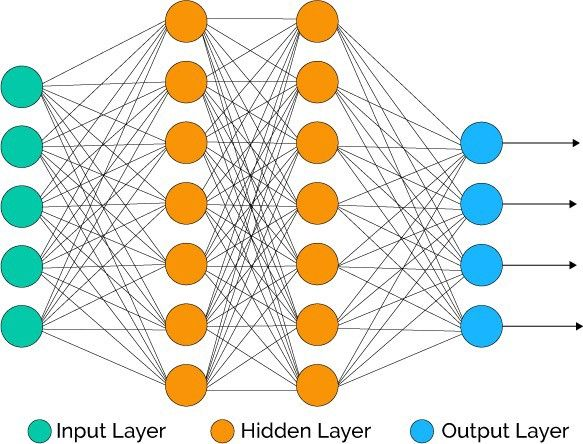
\includegraphics[width=1.0\linewidth]{Chapters/items/ann.jpg}
         
        \label{fig: ann}
    \end{subfigure}
    \caption{Ví dụ mạng nơ-ron nhân tạo đơn giản}
\end{figure}


Quá trình huấn luyện mô hình là quá trình xác định các giá trị của
các trọng số và hệ số tự do. Các giá trị của chúng được khởi tạo với
các giá trị ngẫu nhiên khi bắt đầu huấn luyện. Muốn huấn luyện chúng
ta cần phải định nghĩa bằng hàm lỗi của mạng. Lúc này chúng ta
sẽ nhắc đến hai giá trị đó là ground truth - tức là giá trị
thực tế có trong tập dữ liệu huấn luyện và predict output là
giá trị mà mô hình dự đoán. Lỗi được tính bằng cách sử dụng
hàm loss định nghĩa dựa trên sự khác nhau giữa hai giá trị này.
Có nhiều kiểu định nghĩa hàm loss khác nhau mà chúng ta sẽ thực
hiện trong series này. Làm đến phần nào chúng ta sẽ nói rõ hơn ở
phần đó. Dựa trên gíá trị của hàm đánh giá mất mát được tính toán, các trọng
số trọng số được điều chỉnh tại mỗ bước trong quá trình huấn luyện.
uá trình huấn luyện thực chất là tìm ra các đặc trưng features trong
dữ liệu đầu vào. Các features này là một đại diện tốt hơn so với dữ
liệu thô.


\section{Mô hình mạng neural tích chập (Convolutional neural network - CNN)}

Mạng neural tích chập (CNN) là một trong những mô hình học sâu\cite{repec} tiên tiến phổ biến nhất và
có ảnh hưởng nhất với cộng đồng thị giác máy tính (Computer vision). CNN thường được dùng
trong các bài toán nhận dạng ảnh, phân tích ảnh, xử lý ngôn ngữ tự nhiên dưới dạng ảnh các bước sóng.
Và hầu hết đều cho hiệu quả tốt đến rất tốt.

CNN là một kiến trúc mạng neural sinh ra để xử lý các dữ liệu phi cấu trúc dạng ảnh. Có 2 loại lớp
chính trong CNN: lớp tích chập (Convolutional layer) và lớp gộp (Pooling layer)

\begin{figure}
    \begin{subfigure}{1.\textwidth}
        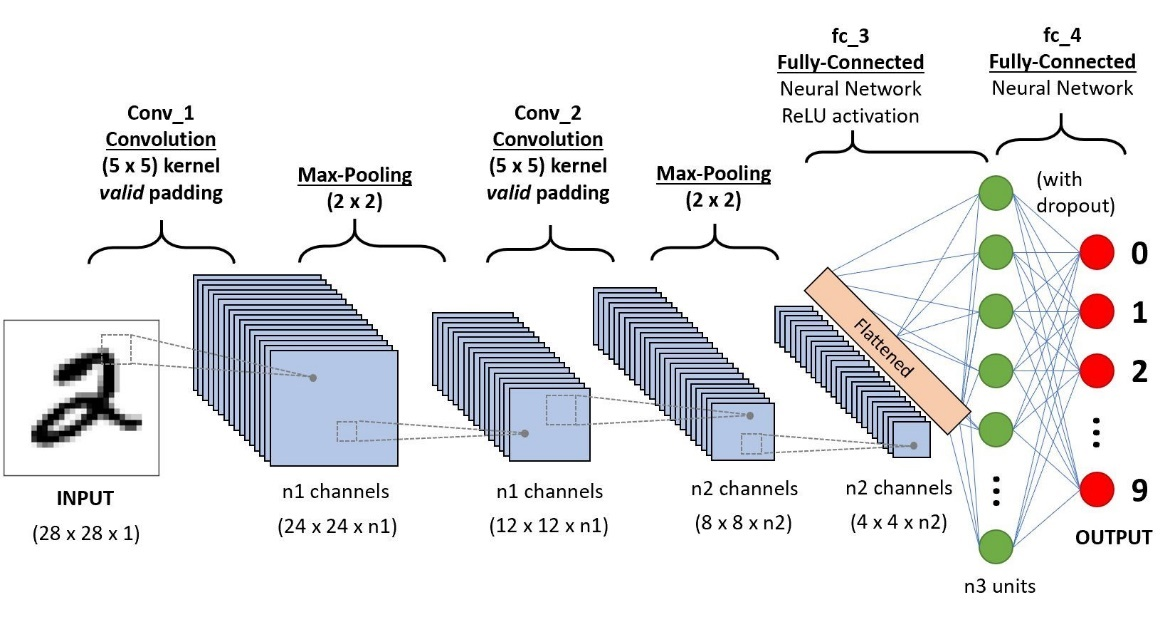
\includegraphics[width=1.\linewidth]{Chapters/items/cnn2_1.jpg}
        \label{fig: chap2_2}
    \end{subfigure}
    \caption{CNN cho bài toán nhận diện chữ số.}
\end{figure}
\subsection{Lớp tích chập}

Lớp tích chập là lớp quan trọng nhất và thường cũng là lớp đầu tiên của của mô hình CNN.
Lớp này có chức năng chính là phát hiện các đặc trưng có tính không gian hiệu quả.
Trong tầng này có 4 đối tượng chính là: ma trận đầu vào, bộ lọc (filters) và trường thụ cảm,
bản đồ đặc trưng (feature map). Lớp tích chập nhận đầu vào là một ma trận 3 chiều và một bộ lọc cần phải học.
Bộ lọc này sẽ trượt qua từng vị trí trên bức ảnh để tính tích chập (convolution)
giữa bộ lọc và phần tương ứng trên bức ảnh. Phần tương ứng này trên bức ảnh gọi là
trường thục cảm (receptive field), tức là vùng mà một neuron có thể nhìn thấy để đưa
ra quyết định, và mà trận cho ra bởi quá trình này được gọi là bản đồ đặc trưng (feature map).

Để hình dung, có thể tưởng tượng, bộ filters giống như các tháp canh trong nhà tù quét
lần lượt qua không gian xung quanh để tìm kiếm tên tù nhân bỏ trốn.
Khi phát hiện tên tù nhân bỏ trốn, thì chuông báo động sẽ reo lên, giống như các bộ lọc
tìm kiếm được đặc trưng nhất định thì tích chập đó sẽ cho giá trị tương ứng.

\begin{enumerate}
    \item Lớp tích chập được coi như xác định đặc trưng
          \begin{itemize}
              \item Lớp tích chập có chức năng chính là phát hiện đặc trưng cụ thể của bức ảnh.
                    Những đặc trưng này bao gồm đặc trưng cơ bản là góc, cạnh, màu sắc, hoặc đặc trưng
                    phức tạp hơn như texture của ảnh. Vì bộ lọc quét qua toàn bộ bức ảnh, nên những
                    đặc trưng này có thể nằm ở vị trí bất kì trong bức ảnh, cho dù ảnh bị xoáy trái/phải
                    thì những đặc trưng này vẫn bị phát hiện.
              \item Ở minh họa dưới, có một bộ lọc 5x5 dùng để phát hiện góc/cạnh, với bộ lọc này
                    chỉ có giá trị một tại các điểm tương ứng một góc cong.
                    \begin{figure}
                        \begin{subfigure}{0.6\textwidth}
                            \begin{center}
                                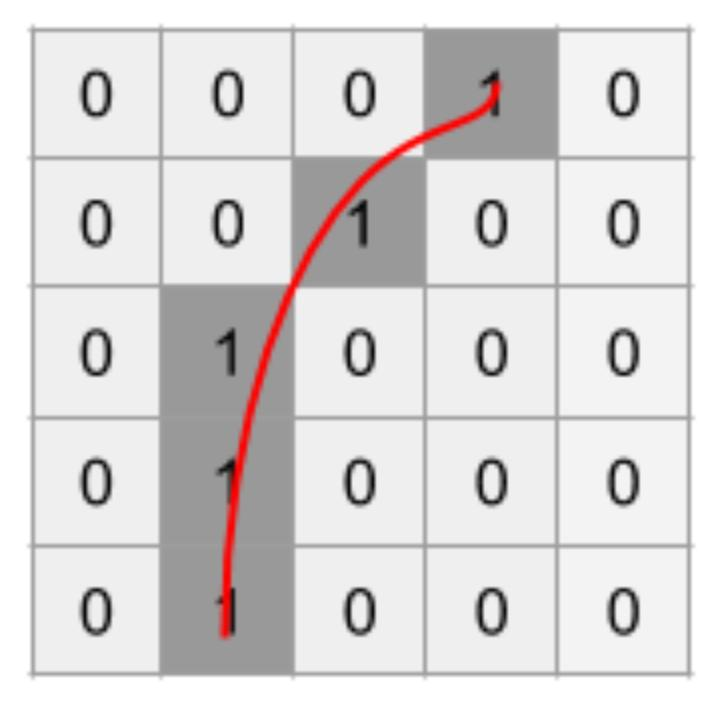
\includegraphics[width=0.6\linewidth]{Chapters/items/chap2_3.jpg}
                            \end{center}
                            \label{fig: chap2_3}
                        \end{subfigure}
                        \caption{Bộ lọc phát hiện cạnh}
                    \end{figure}
              \item Dùng bộ lọc ở trên trược qua ảnh của nhân vật Olaf trong trong bộ phim Frozen.
                    Chúng ta thấy rằng, chỉ ở những vị trí trên bức ảnh có dạng góc như đặc trưng ở
                    bộ lọc thì mới có giá trị lớn trên bản đồ đặc trưng, những vị trí còn lại sẽ cho giá trị
                    thấp hơn. Điều này có nghĩa là, bộ lọc đã phát hiện thành công một dạng góc/cạnh
                    trên dự liệu đầu vào. Tập hơn nhiều bộ lọc sẽ cho phép các bạn phát hiện được
                    nhiều loại đặc trưng khác nhau,và giúp định danh được đối tượng.
                    \begin{figure}
                        \begin{subfigure}{1.\textwidth}
                            \begin{center}
                                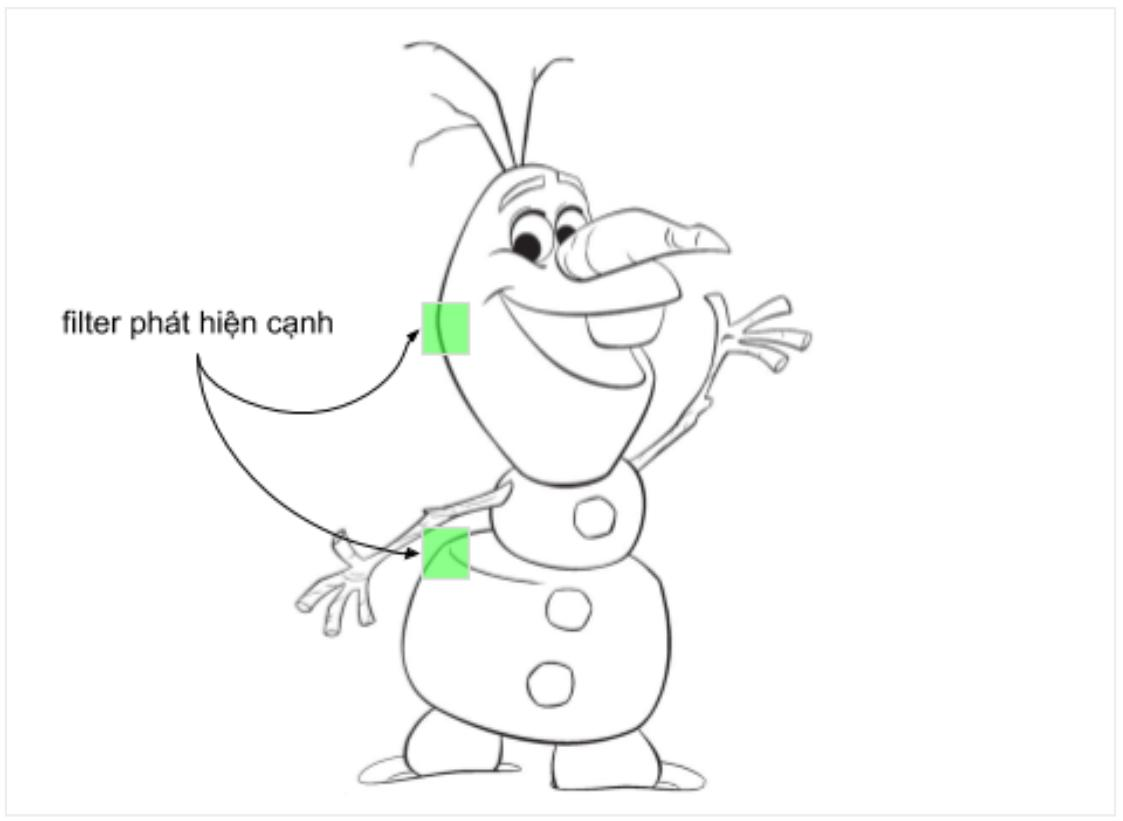
\includegraphics[width=1.\linewidth]{Chapters/items/chap2_4.jpg}
                            \end{center}
                            \label{fig: chap2_4}
                        \end{subfigure}
                        \caption{Bộ lọc phát hiện cạnh}
                    \end{figure}
          \end{itemize}
    \item Các tham số: Kích thước bộ lọc, bước nhảy, lề
          \begin{itemize}
              \item Kích thước bộ lọc là một trong những tham số quan trọng nhất của lớp tích chập.
                    Kích thước này tỉ lệ thuận với số tham số cần học tại mỗi lớp tích chập và
                    là tham số quyết định trường thụ cảm của tầng này. Kích thước phổ biến nhất của bộ lọc
                    là 3x3.
                    \begin{figure}
                        \begin{subfigure}{1.\textwidth}
                            \begin{center}
                                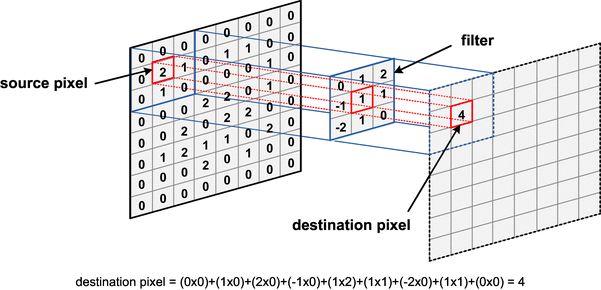
\includegraphics[width=1.\linewidth]{Chapters/items/chap2_5.jpg}
                            \end{center}
                            \label{fig: chap2_5}
                        \end{subfigure}
                        \caption{Cách hoạt động của bộ lọc (filter)}
                    \end{figure}
              \item Kích thước bộ lọc nhỏ được ưu tiên lựa chọn thay kích thước lớn vì những lý do sau đây:
                    \begin{itemize}
                        \item Cho phép nhìn được các vùng nhỏ
                        \item Trích rút được những đặc trưng có tính cục bộ cao
                        \item Phát hiện đặc trưng nhỏ
                        \item Đặc trưng được trích rút sẽ nhiều, đa dạng
                        \item Giảm kích thước ảnh chậm, cho phép mạng sâu hơn
                        \item Chia sẻ trọng số tốt hơn
                    \end{itemize}
              \item Kích thước của bộ lọc sẽ là những số lẻ để kết quả của phép tích chập sẽ nằm ở giữa ma trận
          \end{itemize}
\end{enumerate}

\subsection{Lớp phi tuyến}

Để các mô hình học sâu tìm được mối quan hệ phức tạp giữa các đặc trưng, cũng như tìm được những đặc trưng quan trọng
(là sự kết hợp phi tuyến giữa các đặc trưng cơ bản khác) thì các mối quan hệ đó khó có thể được biểu diễn dưới các hàm tuyến tính
mà cần sự kết hợp phi tuyến tính, chính vì vậy các hàm kích hoạt phi tuyến ra đời nhằm phá vỡ sự tuyến tính của giữa các đặc trưng từ đó tìm
ra các đặc trưng mới quan trọng hơn.

Hiện nay hàm kích hoạt được sử dụng phổ biến nhất là hàm ReLU (Rectified Linear Units). Hàm ReLU được ưa chuộm vì tính đơn giản và cho kết quả tốt hơn
ReLU cũng như những hàm kích hoạt khác, được đặt ngay sau tầng convolution, ReLU sẽ gán những giá trị âm bằng 0 và giữ nguyên giá trị của đầu vào khi lớn hơn 0.

ReLU cũng có một số vấn đề tiềm ẩn như không có đạo hàm tại điểm 0, giá trị của hàm ReLU có thể lớn đến vô cùng và
nếu chúng ta không khởi tạo trọng số cẩn thận, hoặc khởi tạo tỉ lệ học (learning rate) quá lớn thì những neuron ở tầng này sẽ rơi vào trạng thái chết, tức là luôn có giá trị < 0.

\begin{figure}
    \begin{subfigure}{1.\textwidth}
        \begin{center}
            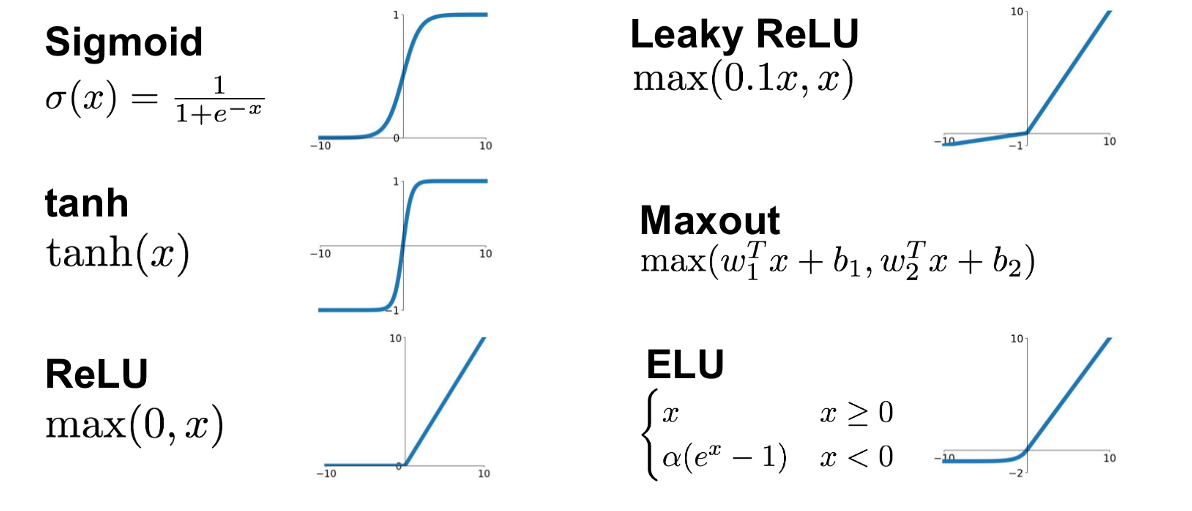
\includegraphics[width=1.\linewidth]{Chapters/items/chap2_6.jpg}
        \end{center}
        \label{fig: chap2_6}
    \end{subfigure}
    \caption{Một số hàm kích hoạt thường được sử dụng}
\end{figure}

\newpage
\subsection{Lớp gộp}

Sau hàm kích hoạt, thông thường chúng ta sử dụng lớp gộp. Một số loại lớp gộp phổ biến như là max-pooling, average pooling,
với chức năng chính là giảm chiều của tầng trước đó. Với một lớp gộp có kích thước 2x2,
các bạn cần phải trượt bộ lọc 2x2 này trên những vùng ảnh có kích thước tương tự rồi sau đó tính giá trị lớn nhất,
hay trung bình cho vùng ảnh đó.

\begin{figure}
    \begin{subfigure}{1.\textwidth}
        \begin{center}
            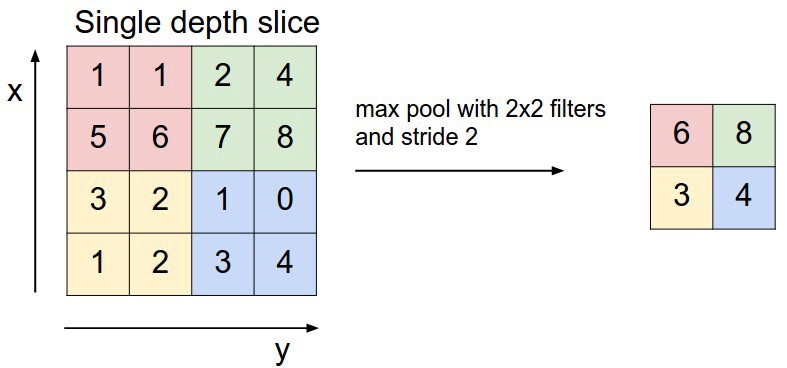
\includegraphics[width=1.\linewidth]{Chapters/items/chap2_7.jpg}
        \end{center}
        \label{fig: chap2_7}
    \end{subfigure}
    \caption{Ví dụ về max-pooling}
\end{figure}

Ý tưởng đằng sau lớp gộp là vị trí tuyết đối của những đặc trưng trong không gian ảnh không
còn cần cần thiết, thay vào đó vị trí tương đối giữ các đặc trưng đã đủ để phân loại đối tượng.
Hơn giảm tầng pooling có khả năng giảm chiều cực kì nhiều, làm hạn chế overfit,
và giảm thời gian huấn luyện tốt.


\subsection{Lớp kết nối đầy đủ}

Lớp cuối cùng của mô hình CNN trong bài toán phân loại ảnh là lớp kết nối đầy đủ.
Lớp này có chức năng chuyển ma trận đặc trưng ở tầng trước thành các vector chứa xác suất của các
đối tượng cần được dự đoán.

Quá trình huấn luyện mô hình CNN cho bài toán phân loại ảnh cũng tương tự như huấn luyện các
mô hình khác. Cần có hàm đánh giá mất mát để tính sai số giữa dự đoán của mô hình và nhãn chính xác,
để sử dụng cơ chế của thuật toán lan truyền ngược (backprobagation) cho quá trình cập nhật trọng số.

\begin{figure}
    \begin{subfigure}{1.\textwidth}
        \begin{center}
            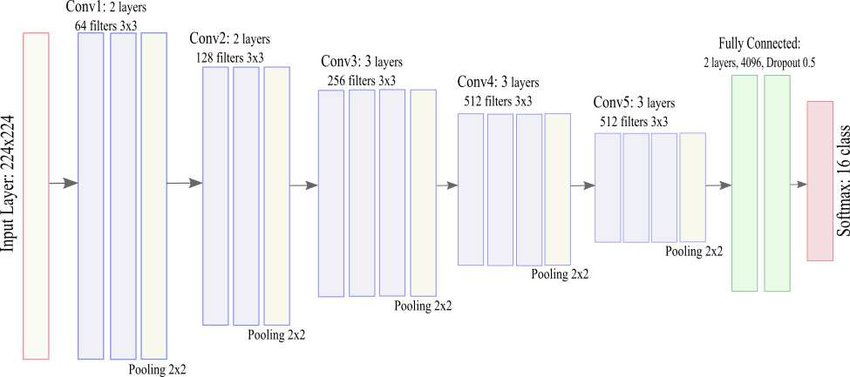
\includegraphics[width=1.\linewidth]{Chapters/items/chap2_8.jpg}
        \end{center}
        \label{fig: chap2_8}
    \end{subfigure}
    \caption{Một CNN đơn giản với đầy đủ các lớp}
\end{figure}

\newpage



\section{Bộ mã hóa tự động (Autoencoder)}

Bộ mã hóa tự động là một kỹ thuật học tập không có giám sát,
trong đó chúng em tận dụng mạng nơ-ron cho nhiệm vụ của học để biểu diễn các tập
giá trị dưới dạng nén và học cách để giải mã dữ liệu từ dạng nén.

Cụ thể, chúng em sẽ thiết kế một kiến trúc mạng nơ-ron nhân tạo sau đó áp đặt một
nút thắt cổ chai trong mạng - điều này đại diện cho sự nén lại một cách tự động.
Mạng này sẽ phải biểu diễn tri thức đầu vào dưới dạng các biểu diễn trong ít
chiều không gian hơn, đây chính là biểu diễn nén của đầu vào.

\begin{figure}
    \begin{subfigure}{0.8\textwidth}
        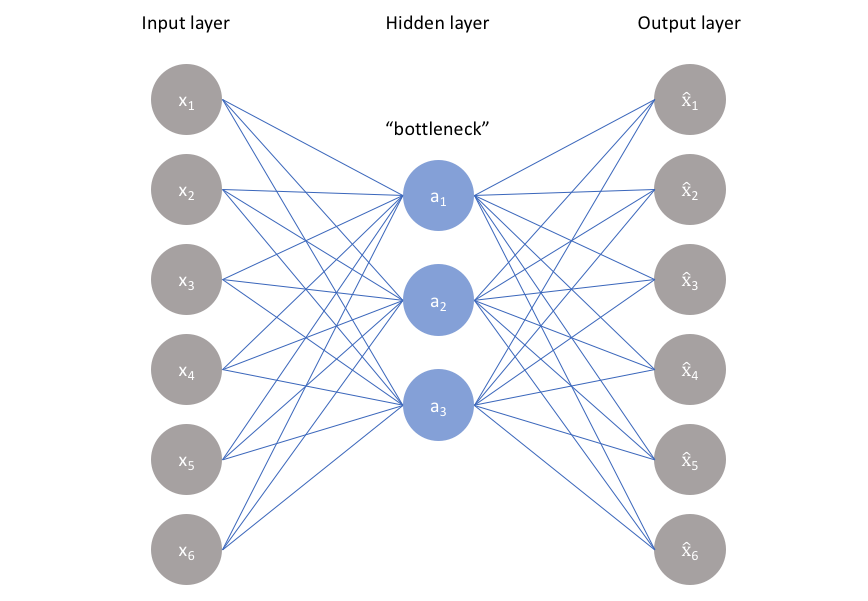
\includegraphics[width=1.0\linewidth]{Chapters/items/autoencoder1.png}
         
        \label{fig: auto1}
    \end{subfigure}
    \caption{Bộ mã hóa tự động.}
\end{figure}

Nếu các tính năng đầu vào từng độc lập của nhau, việc nén này và tái tạo sau đó sẽ là
một nhiệm vụ rất khó khăn. Tuy nhiên, nếu một số loại cấu trúc tồn tại trong dữ liệu
(ví dụ như: mối tương quan giữa các tính năng đầu vào), cấu trúc này có thể được
học và do đó được tận dụng khi buộc đầu vào thông qua nút thắt cổ chai của mạng.

Bộ mã hóa tự động lý tưởng cân bằng những điều sau đây:
\begin{itemize}[leftmargin=1.5cm]
    \item Nhạy cảm với các yếu tố đầu vào đủ để xây dựng lại một cách chính xác.
    \item Đủ nhạy cảm với các đầu vào mà mô hình không chỉ đơn giản là ghi
          nhớ hoặc trang bị quá nhiều dữ liệu đào tạo.
\end{itemize}

Sự đánh đổi này buộc mô hình chỉ duy trì các biến thể trong dữ liệu cần
thiết để cấu trúc lại đầu vào mà không giữ lại các phần dư thừa trong đầu vào.
Đối với hầu hết các trường hợp, điều này liên quan đến việc xây dựng một hàm mất mát
trong đó phải thỏa mãn mô hình của chúng ta nhạy cảm với các yếu tố đầu vào
(ví dụ: xây dựng lại 1 hàm mất mát ${\cal L}\left( {x,\hat x} \right)$ và
thêm một chính quy hóa)


\begin{equation}
    {\cal L}\left( {x,\hat x} \right) + regularizer
\end{equation}

Thông thường, sẽ có thêm một tham số tỷ lệ trước thuật ngữ chính quy để chúng ta
có thể điều chỉnh sự cân bằng giữa hai mục tiêu.

Dưới đây chúng em sẽ trình bày về một số kiến trúc của bộ mã hóa tư động
tiêu chuẩn để áp đặt 2 ràng buộc này và điều chỉnh sự cân bằng.


% \newpage
% \subsection{Cấu trúc bộ mã hóa tự động}
% Một bộ mã hóa tự động có 3 thành phần chính : bộ mã hóa f,
% bộ giải mã g, mô hình xác suất Q

\subsection{Bộ mã hóa tự động chưa hoàn chỉnh}

Kiến trúc đơn giản nhất để xây dựng bộ mã hóa tự động là hạn chế số lượng
nút hiện diện trong (các) lớp ẩn của mạng, hạn chế lượng thông tin có
thể truyền qua mạng. Bằng cách sử dụng các hình phạt mạng theo lỗi xây dựng lại,
mô hình của chúng tôi có thể tìm hiểu các thuộc tính quan trọng nhất của dữ
liệu đầu vào và cách tái tạo tốt nhất dữ liệu đầu vào ban đầu từ trạng thái
"được mã hóa". Lý tưởng nhất là bảng mã này sẽ tìm hiểu và mô tả các thuộc
tính tiềm ẩn của dữ liệu đầu vào.

\begin{figure}
    \begin{subfigure}{0.8\textwidth}
        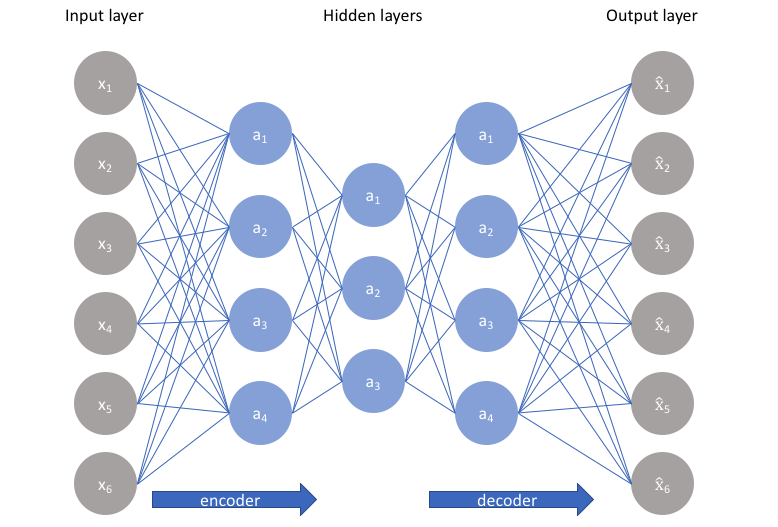
\includegraphics[width=1.\linewidth]{Chapters/items/auto2.jpg}
         
        \label{fig: auto2}
    \end{subfigure}
    \caption{Mô tả mô hình bộ mã hóa tự động chưa hoàn chỉnh.}
\end{figure}

Bởi vì mạng nơ-ron có khả năng học các mối quan hệ phi tuyến,
điều này có thể được coi là một sự tổng quát hóa (phi tuyến)
mạnh mẽ hơn của PCA (kĩ thuật giảm chiều dữ liệu tuyến tính)

\newpage
Trong khi PCA cố gắng khám phá một siêu phẳng có chiều thấp hơn
mô tả dữ liệu ban đầu, thì các bộ mã hóa tự động có khả năng học các
đa tạp phi tuyến (đa tạp được định nghĩa theo thuật ngữ đơn giản
là liên tục, không giao nhau bề mặt). Sự khác biệt giữa hai cách
tiếp cận này được hình dung bên dưới.

\begin{figure}
    \begin{subfigure}{0.5\textwidth}
        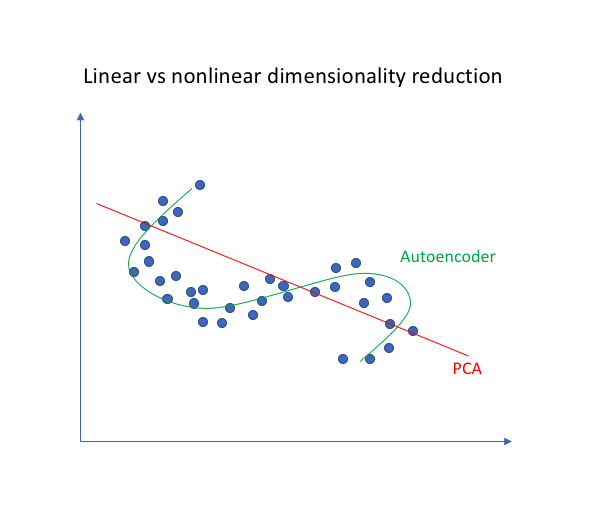
\includegraphics[width=1.\linewidth]{Chapters/items/auto3.jpg}
         
        \label{fig: auto3}
    \end{subfigure}
    \caption{Mô tả mô hình bộ mã hóa tự động chưa hoàn chỉnh.}
\end{figure}

Một bộ mã hóa tự động chưa hoàn chỉnh không có thuật ngữ chính quy
rõ ràng - chúng tôi chỉ đào tạo mô hình của mình theo sự mất mát
khi xây dựng lại. Do đó, cách duy nhất của chúng tôi để đảm bảo rằng
mô hình không ghi nhớ dữ liệu đầu vào là đảm bảo rằng chúng tôi đã
hạn chế đủ số lượng các nút trong (các) lớp ẩn.

Đối với các bộ mã hóa tự động sâu, chúng ta cũng phải lưu ý về dung
lượng của bộ mã hóa và các kiểu máy giải mã của chúng ta.
Ngay cả khi "lớp nút cổ chai" chỉ là một nút ẩn, mô hình của
chúng tôi vẫn có thể ghi nhớ dữ liệu huấn luyện với điều kiện là
các mô hình bộ mã hóa và giải mã có đủ khả năng để học một số chức
năng tùy ý có thể ánh xạ dữ liệu thành một chỉ mục.

\subsection{Bộ mã hóa tự động thưa thớt}

Các bộ mã hóa tự động thưa thớt cung cấp cho chúng ta một phương pháp
thay thế để giới thiệu một nút thắt cổ chai thông tin mà không
yêu cầu giảm số lượng nút ở các lớp ẩn của chúng ta. Thay vào đó,
chúng tôi sẽ xây dựng hàm mất mát của chúng tôi để chúng tôi
xử phạt các hàm kích hoạt trong một lớp. Đối với bất kỳ quan sát
nhất định nào, chúng ta sẽ khuyến khích mạng của mình học cách mã hóa và
giải mã chỉ dựa vào việc kích hoạt một số lượng nhỏ nơ-ron.

\begin{figure}
    \begin{subfigure}{0.8\textwidth}
        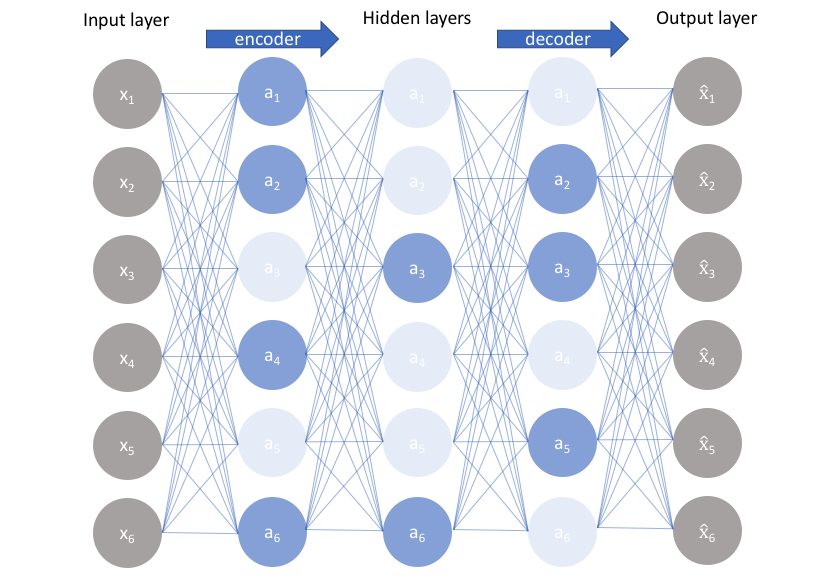
\includegraphics[width=1.\linewidth]{Chapters/items/auto4.jpg}
         
        \label{fig: auto4}
    \end{subfigure}
    \caption{Mô tả mô hình bộ mã hóa tự động chưa hoàn chỉnh.}
\end{figure}

\newpage
Một bộ mã hóa tự động thưa thớt chung được hiển thị bên trên nơi
độ mờ của một nút tương ứng với mức độ kích hoạt. Điều quan
trọng cần lưu ý là các nút riêng lẻ của một mô hình được đào
tạo kích hoạt phụ thuộc vào dữ liệu , các đầu vào khác nhau
sẽ dẫn đến việc kích hoạt các nút khác nhau thông qua mạng.

Một kết quả của thực tế này là chúng tôi cho phép mạng của
mình nhạy cảm với các nút lớp ẩn riêng lẻ đối với các thuộc
tính cụ thể của dữ liệu đầu vào. Trong khi một bộ mã hóa tự động
chưa hoàn chỉnh sẽ sử dụng toàn bộ mạng cho mỗi lần quan sát,
một bộ mã hóa tự động thưa thớt sẽ buộc phải kích hoạt có chọn lọc
các vùng của mạng tùy thuộc vào dữ liệu đầu vào. Do đó, chúng
tôi đã giới hạn khả năng ghi nhớ dữ liệu đầu vào của mạng mà
không giới hạn khả năng mạng trích xuất các tính năng từ dữ liệu.

Điều này cho phép chúng tôi xem xét biểu diễn trạng thái tiềm ẩn
và quy định của mạng một cách riêng biệt, do đó chúng tôi có thể
chọn biểu diễn trạng thái tiềm ẩn (tức là kích thước mã hóa) phù
hợp với những gì có ý nghĩa với ngữ cảnh của dữ liệu trong khi áp
đặt chính quy bởi ràng buộc thưa thớt.

Có hai cách chính mà chúng ta có thể áp đặt hạn chế thưa thớt này;
cả hai đều liên quan đến việc đo lường các kích hoạt lớp ẩn
cho mỗi lô đào tạo và thêm một số thuật ngữ vào hàm mất mát để
xử phạt các kích hoạt quá mức. Các cách này là:

\begin{itemize}[leftmargin=1.5cm]
    \item \textbf{L1 Regularization}: Chúng ta có thể thêm một thuật ngữ vào hàm mất mát
          để phạt giá trị tuyệt đối của vector kích hoạt \textit{a} trong lớp \textit{h} với quan sát \textit{i}, được chia tỉ lệ
          bằng 1 tham số điều chỉnh \textit{$\lambda$}
          \begin{equation}
              {\cal L}\left( {x,\hat x} \right) +  \lambda \sum\limits_i {\left| {a_i^{\left( h \right)}} \right|}
          \end{equation}
    \item \textbf{KL-phân kỳ} Về bản chất, KL-phân kỳ là thước đo sự
          khác biệt giữa hai phân phối xác suất. Chúng ta có thể xác định
          tham số thưa thớt \textit{p} biểu thị kích hoạt trung bình của
          một nơ-ron trên một tập hợp các mẫu. Kỳ vọng này có thể được tính là:
          \begin{equation}
              {{\hat \rho }_ j} = \frac{1}{m}\sum\limits_{i} {\left[ {a_i^{\left( h \right)}\left( x \right)} \right]}
          \end{equation}
          trong đó chỉ số con \textit{i} biểu thị nơ-ron cụ thể trong lớp \textit{h}, tính tổng các kích hoạt
          cho các quan sát huấn luyện \textit{m} được ký hiệu riêng lẻ là \textit{x}.

\end{itemize}

\subsection{Bộ mã hóa tự động giảm nhiễu}

Như ở phần giới thiệu, bộ mã hóa tự động chính là một mạng
nơ-ron được đào tạo
trong đó đầu vào giống hệt đầu ra và mô hình có nghiệm vụ tái
tạo đầu vào càng
chặt chẽ càng tốt khi chuyển qua thông tin ở lớp thắt cổ chai.
Một cách tiếp cận khác hướng tới việc phát triển một mô hình
tổng quát hóa là làm nhiễu một chút dữ liệu đầu vào nhưng vẫn
duy trì dữ liệu không bị gián đoạn làm đầu ra mục tiêu của mô hình.

\begin{figure}
    \begin{subfigure}{0.8\textwidth}
        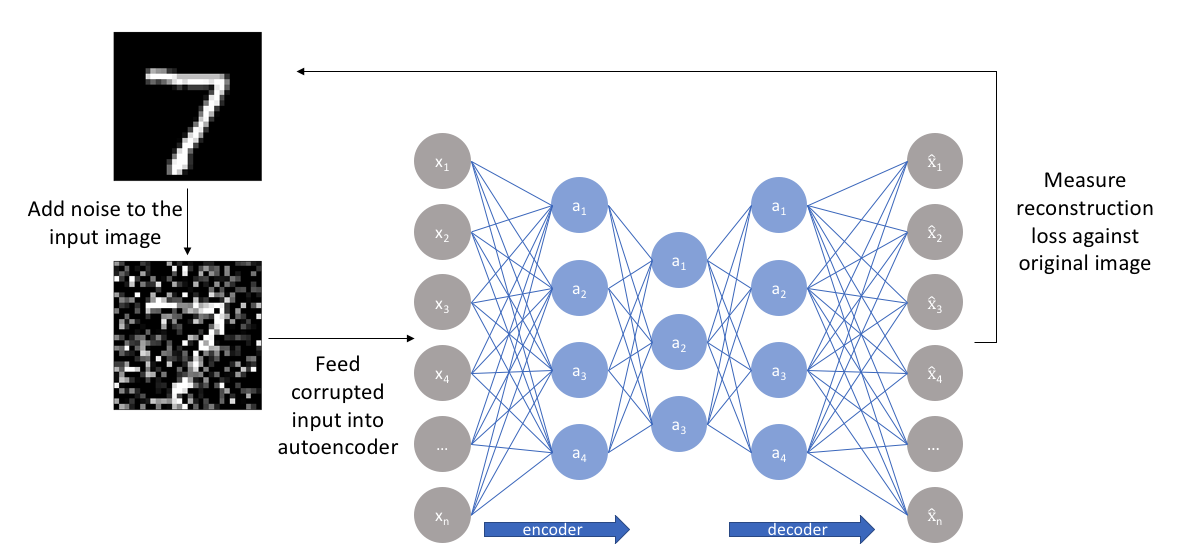
\includegraphics[width=1.\linewidth]{Chapters/items/auto5.jpg}
         
        \label{fig: auto5}
    \end{subfigure}
    \caption{Mô tả mô hình bộ mã hóa tự động chưa hoàn chỉnh.}
\end{figure}

Với cách tiếp cận này, mô hình không thể đơn giản
phát triển một ánh xạ ghi nhớ dữ liệu đào tạo vì đầu vào và đầu
ra mục tiêu không còn giống nhau. Thay vào đó, mô
hình học một trường vectơ để ánh xạ dữ liệu đầu vào tới một đa
tạp có chiều thấp hơn (nhớ lại từ hình ảnh trước đây của tôi rằng
một đa tạp mô tả vùng mật độ cao nơi dữ liệu đầu vào tập trung).

\section{Ngôn ngữ lập trình Python và thư viện PyTorch}

\subsection{Ngôn ngữ lập trình Python}

Python là ngôn ngữ lập trình có mục đích chung được bắt đầu bởi Guido van Rossum,
nó trở nên rất phổ biến rất nhanh trong thời gian gần đây, chủ yếu vì tính đơn giản
và khả năng đọc mã của nó. Nó cho phép lập trình viên thể hiện ý tưởng trong ít dòng
mã hơn mà không làm giảm khả năng đọc.

So với các ngôn ngữ như C/C++, Python chậm hơn. Điều đó nói rằng, Python có thể dễ dàng
được mở rộng với C/C++, cho phép chúng ta viết mã chuyên sâu tính toán trong C/C++
và tạo các trình bao bọc Python có thể được sử dụng làm mô-đun Python.
Điều này mang lại cho chúng ta hai lợi thế: thứ nhất, mã nhanh như mã C/C++ gốc
(vì đây là mã C++ thực tế hoạt động ở chế độ nền) và thứ hai, mã dễ dàng hơn trong
Python so với C/C++. OpenCV - Python là một trình bao bọc Python để thực hiện OpenCV C++
ban đầu.

\subsection{Thư viện PyTorch}

PyTorch là một thư viện hỗ trợ tạo ra các mô hình mạng nơ-ron nhân tạo và sử
dụng chúng trong các ứng dụng khác nhau. Trên thực tế PyTorch chính là một
gói hỗ trợ tính toán khoa học (scientific computing) như tài liệu chính
thức của PyTorch đã đề cập

PyTorch, tương tự như Python, nó được thiết kế tập trung vào tính dễ
sử dụng và thậm chí người dùng có kiến thức lập trình rất cơ bản cũng có thể
sử dụng nó trong các dự án có liên quan đến học sâu.


